\section{Step 4: 入力フィールドの変更へ反応する}

Webディベロッパーの皆さんはDOM(Document Object Model, ブラウザの機能へアクセスするAPIのセット)の扱いに慣れているかと思います.しかし,多くの人はブラウザのインターフェースを触りやすくしたり,ブラウザ間の相違をなくすためにjQueryを使っているかと思います.jQueryがDOMをJavaScriptから利用しやすくするように,DartもDartから利用しやすくするようにHTML libraryを提供しています.

HTML library\footnote{\url{http://api.dartlang.org/html.html}}は<div>,<p>などのWebページ上の要素(Element)に対するアクセス手段を提供します.ページ上の要素を見つけたり,新しい要素を作成したり,テキストを変更したり,様々なことができます.また,HTMLの新しい機能であるIndexedDBやApplication Cache,そしてWebGLなどへもHTML libraryを利用してアクセスすることができます.

WebアプリケーションはWebページ上では単一のUIスレッド上で動作します.\footnote{WebWorkerなどの例外はあります.しかし,これらの応用的なトピックについてはここでは触れません.}目に見えて動作が固まったり遅れることを最小化するために,マウスクリックやボタンが押されたことなどのイベントに対する応答はコールバック(Callback)として起こります.例えば入力フィールドなどのページ上の要素のハンドル(Handle)を取得すれば,特定のイベントの時に実行される関数を登録することができます.(例えば,''on change''イベントなど)

\subsection{目標}

\begin{enumerate}
\item ライブラリをImportする
\item CSSセレクタを利用してHTMLページ上の要素を見つける.
\item HTML要素(HTML element)のイベントに関連付ける
\item レキシカルクロージャ(Lexical Closure), インラインコールバック(Inline Callback), そして単一行関数(One-Line Function)を利用する
\item 入力フィールドを有効化したり無効化する
\item 入力要素の内容を取得する
\item Dartのゲッター(Getter)が実際にどのように動作するかを確認する
\item どのメソッドが利用できるかを知るためにDart Editorのコード補完を利用する
\end{enumerate}

\subsection{コード}

もし,作業につまづいた場合はstep04のフォルダの内容をstart-hereフォルダにコピーすることで,この部分の作業内容を終わらせた状態にすることができます.

\subsection{ウォークスルー}

コードにとりかかる前に,Dart Editorが持つ生産的できっと役に立つ機能の一つを紹介します.コード補完(Code Completion)です.型情報(直接的なアノテーション型宣言(Type Annotations),単純な型推論,また,型伝播(Type Propagation))を利用して,Dart Editorは利用可能なメソッドやオブジェクト上のフィールドのリストを表示します.Macをお使いの場合であれば,コントロールとスペースを同時に押すことでコード補完を呼び出すことができます.

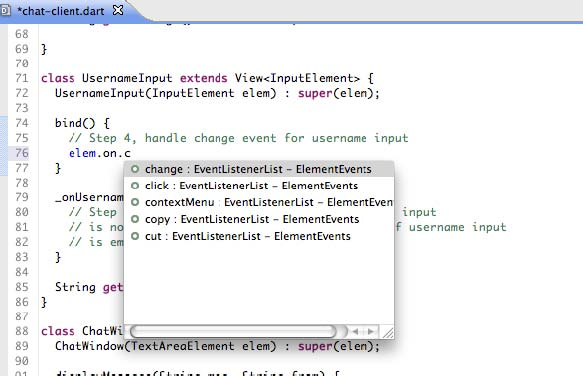
\includegraphics{step4/img_40.jpg}

このステップやこれ以降のステップでコードを書くとき,コード補完を試してみてください.もし,Dart Editorが思ったような候補を表示してくれない場合はアノテーション型宣言を対象のオブジェクトに追加してみてください.

(チップ: コード補完を利用しようとしていて,正しい候補を提供してくれない場合,Send Feedbackボタンを押してDartチームに知らせてください.その際,補完しようとしているコードのスニペットを一緒に送ってください.)

\subsubsection{HTML内の要素を特定する}

HTML libraryを追加して,ページ上に存在する要素を見つけ,イベントを登録し,DOM要素を操作しましょう.

$ client/index.html $を開きます.2つの\verb|<input>|タグと\verb|<textarea>|タグのIDを特定してください.例えば,

\begin{verbatim}
// client/index.html
<textarea id="chat-display" rows="10" cols="100" disabled></textarea>
...
<input id="chat-username" name="chat-username" type="text">
...
<input id="chat-message" name="chat-message" type="text" disabled
value="enter username...">
\end{verbatim}

特定の要素を簡単に見つけることができるようにするために,HTML要素のIDはドキュメント内において固有です.

\subsubsection{dart:htmlライブラリがインポートされたことを確認する}

3つのIDを確認したら,DartのHTML libraryを使ってそれらの要素のハンドルを取得することができます.$ client/chat-client.dart $を開いてファイルの先頭までスクロールしてください.

dart:htmlのインポート文は既に追加されていることがわかると思います.今回,エラーを表示させないために私たちは追加しておきましたが,普段は自分で追加する必要があります.

\begin{verbatim}
// client/chat-client.dart
#library('chat-client');
#import('dart:html');
...
// This is already here, just pointing it out. :)
...
\end{verbatim}

\subsubsection{HTMLの要素を見つける}

dart:htmlのトップレベルの関数であるquery(String selector)\footnote{\url{http://api.dartlang.org/docs/continuous/dart\_html.html\#query}}を利用して,HTMLページ内の要素を見つけます.query()関数はCSSセレクタを引数として取り,マッチした単一の要素を返します.(queryAll()\footnote{\url{http://api.dartlang.org/docs/continuous/dart\_html.html\#queryAll}}がすべての要素を返す関数として存在します.)

CSSセレクタ\footnote{\url{https://developer.mozilla.org/en/CSS/Getting\_Started/Selectors}}はHTMLページ上の要素をとても的確に示すことができます.IDやクラス名,属性値,DOM内における位置やその他の条件から要素を見つけることができます.このステップでは要素のIDをセレクタとして利用します.例えば,$ \#the-id $と書かれたCSSセレクタはIDが$ the-id $であるHTML要素を探します.

$ client/index.html $から3つの要素を既に見つけていると思います.次のステップは,$ client/chat-client.dart $を下へスクロールしていき,main()メソッドを見つけてください.IDやCSSセレクタ,そして,query()関数について知っていることを利用して,それぞれのHTML要素をDartのオブジェクトに対応付けましょう.

\begin{verbatim}
/ client/chat-client.dart
...
main() {
// Step 4: Identify elements by ID.
TextAreaElement chatElem = query('#chat-display');
InputElement usernameElem = query('#chat-username');
InputElement messageElem = query('#chat-message');
chatWindow = new ChatWindow(chatElem);
usernameInput = new UsernameInput(usernameElem);
messageInput = new MessageInput(messageElem);
...
\end{verbatim}

$\bf{発展的な内容:}$ 明察な読者の方はquery()メソッドは単一の要素(Element\footnote{\url{http://api.dartlang.org/html/Element.html}})を返すが,返り値はより詳細な型(TextAreaElement\footnote{\url{http://api.dartlang.org/html/TextAreaElement.html}} and InputElement\footnote{\url{http://api.dartlang.org/html/InputElement.html}})によりアノテートされていることに気づくでしょう.Dartでは''ダウンキャスト''\footnote{訳者注|ダウンキャストとは基底クラスから派生クラスへの型変換. - Wikipedia 型変換 \url{http://ja.wikipedia.org/wiki/\%E5\%9E\%8B\%E5\%A4\%89\%E6\%8F\%9B\#.E3.83.80.E3.82.A6.E3.83.B3.E3.82.AD.E3.83.A3.E3.82.B9.E3.83.88}} が許されています.これは追加的な型づけをもつシステムでは自然なことで,また,これは''疑わしきは罰せず(innocent until proven guilty)''のプログラミングスタイルを推奨します.アノテーション型宣言が期待される戻り値の型のヒエラルキーの中のものである限り,Dartのツールは警告を発しません.

また,ChatWindow,UsernameInputやMessageInputがどのようにしてコンストラクタでDOMの要素を受け取っているのかも分かると思います.以下に例を示しておきます.

\begin{verbatim}
// client/chat-client.dart
...
class MessageInput extends View<InputElement> {
MessageInput(InputElement elem) : super(elem);
...
\end{verbatim}

\subsubsection{レキシカルクロージャを利用してイベントを紐付ける}

ここではHTML要素のイベントにどのようにして関数を紐付けるのかを学びます.特にユーザー名入力フィールドとメッセージ入力フィールドの2つの''on change''イベントに対してイベントハンドラを紐付けます.単一行コールバック関数(simple one-line callback function)を使う場合,次の1行の形式で示せます:

\begin{verbatim}
element.on.event.add((event) => handleTheEvent())
\end{verbatim}

eventにはマウスクリック,ボタンの押下,値の変化など様々な動作や状態の変化を指定することができます.

チップ: APIドキュメントのElementEvents\footnote{\url{http://api.dartlang.org/html/ElementEvents.html}}を見ると要素に対して利用可能なすべてのイベントを確認できます.

上で使われている単一行間数の文法である\verb|=>|は次の文の短縮形です.

\begin{verbatim}
element.on.event.add((event) {
return handleTheEvent();
});
\end{verbatim}

\verb|=>|はコールバックでの利用に限定されたものではありません.単一行関数が利用できるところであれば,どこでも利用することができます.例えば,これは単一行関数を利用した簡単なクラスです:

\begin{verbatim}
// for illustrative purposes only, not part of the codelab
class Person {
String firstName, lastName;
Person(this.firstName, this.lastName);
String toString() => '$firstName $lastName';
}
\end{verbatim}

Dartのレキシカルクロージャはネストした関数やコールバックを書くことを簡単にします.レキシカルスコープ内の変数に対してコールバック関数の中からアクセスすることができます.また,''this''オブジェクトでさえレキシカルスコープごとに定義されます.

発展的なトピック: レキシカルスコープはプログラム構造に渡るスコープを定義します.''波括弧をたどる''だけでどのオブジェクトや変数がスコープの中にいるのか知ることができます.また,スコープはプログラムの動作に応じて変わることはありません.次のコードはレキシカルスコープのいくつかの例です:

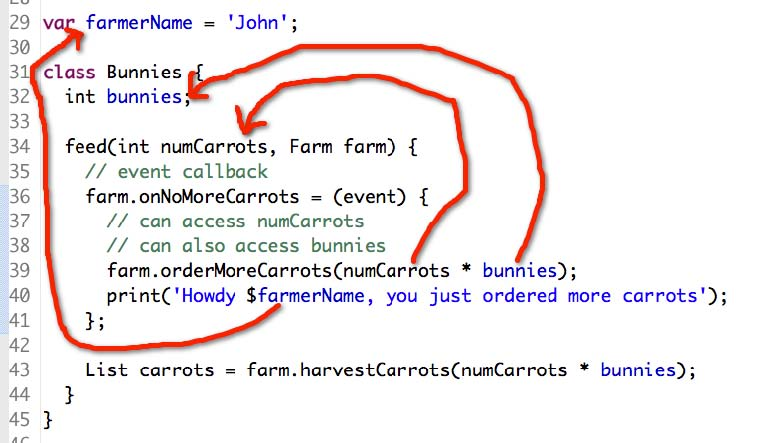
\includegraphics{step4/img_45.jpg}

onNoMoreCarrotsコールバックハンドラーがnumCarrots,bunnies,そしてfarmerNameにアクセスできることが分かると思います.

ユーザー名入力フィールドの値変化イベントで動作するコードを追加します.ユーザー名フィールドが空の時は,メッセージ入力フィールドは無効化されています.ユーザー名入力フィールドに値が入力されている場合は,メッセージフィールドは有効化されます.

\subsubsection{ユーザー名の変更をハンドルする}

$ client/chat-client.dart $を開き,UsernameInputクラスを見つけます.イベントハンドラをUsernameInputのbind()メソッドの内側に追加します.

\begin{verbatim}
// client/chat-client.dart
class UsernameInput extends View<InputElement> {
UsernameInput(InputElement elem) : super(elem);
bind() {
// Step 4: Handle change event for username input.
elem.on.change.add((e) => _onUsernameChange());
}
...
\end{verbatim}

次に\_onUsernameChange()の中にユーザー名フィールドが空でない場合はメッセージ入力フィールドを有効化させるコードを追加します.

\begin{verbatim}
// client/chat-client.dart
_onUsernameChange() {
// Step 4: Enable the message input if username input
// is not empty, or disable the message input if username input
// is empty.
if (!elem.value.isEmpty()) {
messageInput.enable();
} else {
messageInput.disable();
}
}
...
\end{verbatim}

入力要素の値フィールド\footnote{\url{http://api.dartlang.org/html/InputElement.html#value}}は入力フィールドの内容を取得するために使われていることがわかります.isEmpty()\footnote{\url{http://api.dartlang.org/dart_core/String.html#isEmpty}}は文字列に対して利用でき,0文字の文字列の場合にtrueを返します.

MessageInputのインスタンに対してenable()とdisable()メソッドが呼び出されています.MessageInputはこのチャットアプリケーションのために私たちが作成したクラスです.それらのメソッドの実装をチェックしてみてください.

\subsubsection{メッセージ入力フィールドの変更をハンドルする}

メッセージ入力フィールドの取り扱いの仕組みも似ています.メッセージ入力フィールドが変化したら,次の3つのことをすれば良いのです:

\begin{enumerate}
\item chat connectionを経由してメッセージを送ります.
\item チャットウインドウにメッセージを表示します.
\item メッセージ入力フィールドを空にします.
\end{enumerate}

MessageInputクラスを見つけて次のコードを追加してください:

\begin{verbatim}
// client/chat-client.dart
class MessageInput extends View<InputElement> {
MessageInput(InputElement elem) : super(elem);
bind() {
// Step 4: When the message input changes,
// send the message, display the message, and clear the message input.
elem.on.change.add((e) {
connection.send(usernameInput.username, message);
chatWindow.displayMessage(message, usernameInput.username);
elem.value = '';
});
}
\end{verbatim}

connection.send()にmessageが渡されていることに気づくと思います.messageはMessageInputの中で定義されているゲッターメソッドです:

\begin{verbatim}
class MessageInput extends View<InputElement> {
...
String get message() => elem.value;
...
}
\end{verbatim}

発展したトピック: ゲッターはフィールドに似たメソッドで呼び出しの時に()が必要ありません.ゲッターとセッター\footnote{\url{http://www.dartlang.org/docs/language-tour/#classes-getters-and-setters}}は上級のAPI設計においてプロパティをカプセル化し単純なパブリックなフィールドにリファクタリングすることを手助けすることを意図されています.

\subsection{上級編}

\begin{enumerate}
\item 入力フィールドが変更されたときではなく,送信ボタンが押された時に送信するようにしましょう.ボタンを追加し,ラベルをつけ,クリックイベントに応答します.
\item チャットウインドウでメッセージが表示される際にタイムスタンプを表示しましょう.(ヒント: dart:coreのDate\footnote{\url{http://api.dartlang.org/dart_core/Date.html}}を調べてみてください.)
\end{enumerate}
